\documentclass[10pt]{article}
\usepackage{mathtools}
\usepackage[margin=1.25in]{geometry}
\begin{document}
\vspace*{\fill}
\begin{Huge}
\begin{center}
Ayush Jain (UNI : aj2672)\\
COMS W4180 Network Security\\
Written Assignment 3\\
\end{center}
\end{Huge}
\vspace*{\fill}
\newpage
\section{Problem 1}
\textbf{a.} All these rules use the stateless packet filtering approach to approach identify malicious packets. The rules form an Access Control List(ACL) which defines actions based on destination and source ip address and ports of packets. These rules are in the Network Intrusion Detection System(NIDS) mode of Snort.\\\\\\
\textbf{b.} Two problems with this type of approach are:
\begin{itemize}
\item Such rules can allow packets that make no sense. For example, a packet with destination port = 80 and ACK bit set may be allowed by the iptable before a TCP connection is even established.
\item Stateless packet filters cannot support actions based on quantity, i.e. the number of packets from a particular source. 
\end{itemize}
\section{Problem 2}
\begin{enumerate}
\item[(a)]
iptables -A INPUT -i eth0 200.168.20.0.10/12 -j DROP\\
iptables -A INPUT -i eth0 200.168.20.0.12/30 -j DROP\\
iptables -A INPUT -i eth0 200.168.20.0.16/28 -j DROP\\
iptables -A INPUT -i eth0 200.168.20.0.32/29 -j DROP\\
iptables -A INPUT -i eth0 200.168.20.0.40/32 -j DROP\\
The five rows block the traffic from IPs 200.168.20.0.10-11, 200.168.20.0.12-15, 200.168.20.0.16-31, 200.168.20.0.32-39 and 200.168.20.0.40 respectively.
\item[(b)] iptables -A INPUT -i eth0 128.124.0.0/16 -j ACCEPT\\
iptables -A INPUT -i eth0 -j DROP
\item[(c)] iptables -A INPUT -i eth0 -p tcp –dport 80 -j ACCEPT\\
iptables -A INPUT -i eth0 -p tcp –dport 8080 -j ACCEPT\\
iptables -A INPUT -i eth0 -j DROP
\item[(d)] iptables -A OUTPUT -d SERVERBOB –dport 22 -j ACCEPT
\end{enumerate}
\section{Problem 3}
No, having a network where 4 nodes are participating as routers in an onion routing network is of no use. The optimal choice of the number of routers in such a network is three. Let us look at this in more detail to understand why.\\\\
Let us go our way up from one node to understand why three is the optimal choice. If we have only one router then it is of no use because it knows both the sender and the recipient of the data. Also we have only one layer of encryption which can be decrypted by this node and hence this node has full access to the data.\\\\
If we consider a network of two routers, then the first node has information about where data is coming from and also knows the second node from where the data will flow out to the recipient. This makes it easy for traffic correlation.\\\\
However, if we have three intermediate routers, the first one only has the incoming information, the second router does not know any information of the sender and receiver and third router has information only of the data going out. This is the optimal choice. If we add any more nodes we are just increasing the number of intermediate nodes which have no information of incoming or outgoing data. This does not help maintain anonymity but only increases latency. Hence, three intermediate routers is the optimum choice for an onion routing service.
\section{Problem 4}
A nmap run on my own laptop gives the following output. As shown, it is unable to detect the OS, but gives a fingerprint of the OS. It detects four open ports. 
\begin{itemize}
\item 80 - running the Apache default webpage.
\item 631 - running CUPS webpage
\item 3306 - running a MySQL server
\item 5432 - running a PostgreSQL server
\end{itemize}
\begin{figure}[ht!]
\centering
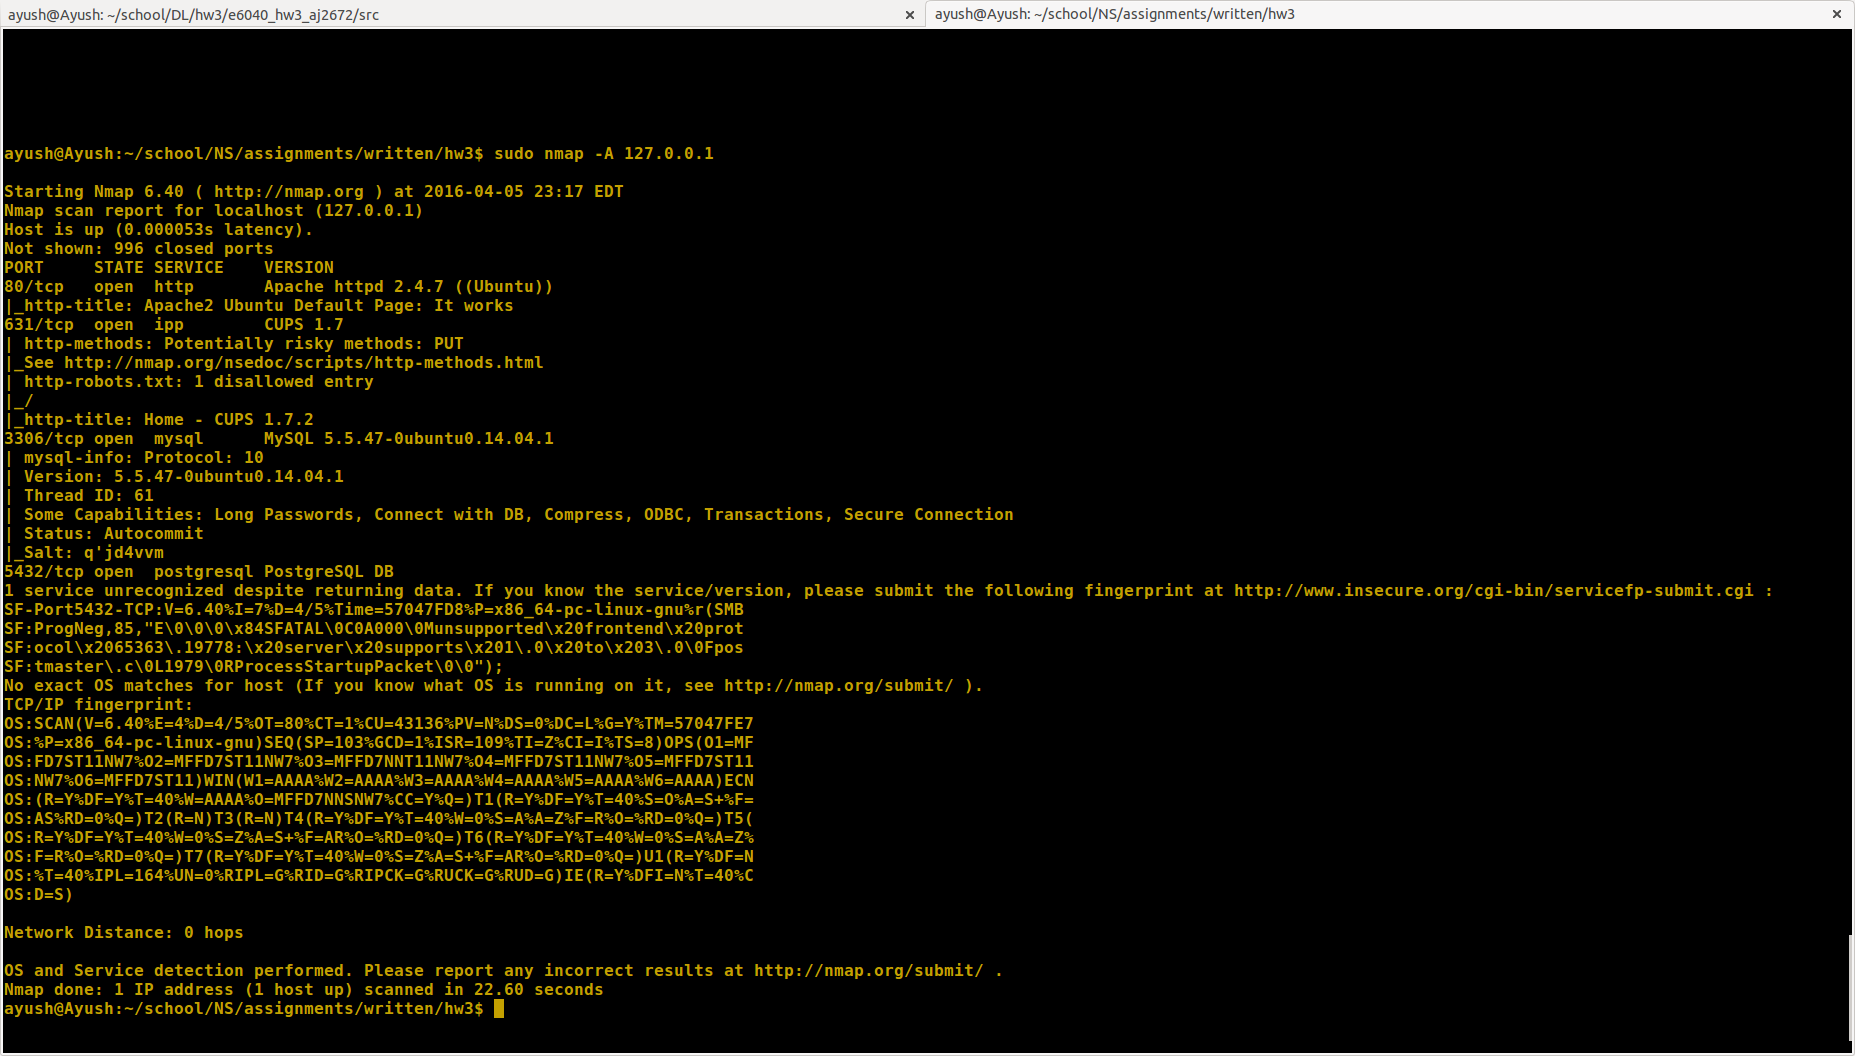
\includegraphics[width=150mm]{nmap.png}
\end{figure}
\section{Problem 5}
Star topology is the easiest botnet topology to disable once the master(s) are discovered. This is because the star topology has only one central master(C\&C resource) that communicates to all the other botnet agents. If this central resource is caught and disabled the entire system is effectively neutered. All the other topologies have more than one central master(s) and are harder to disable.
\section{Problem 6}
\textbf{a.} GMBot is an android banking trojan. It uses dynamic application overlay which is similar in principle to the webinjects infrastructure. When GMBot sees that a banking application is open it displays a window on top of the banking application. The user enters his banking credentials assuming that it is the banking application asking for them and hence considers it safe which are then stolen by the malicious application.\\\\\\
\textbf{b.} The Angler used the Diffie-Hellman algorithm cryptographic algorithm. It was used  to get a structure with the shellcode of the recent exploits for vulnerabilities for the Internet Explorer 11 browser and Adobe Flash. Most likely, the goal of the threat actors was to create difficulties in firewall detection of the exploit as firewalls cannot decipher a shellcode and exploit by the means of the intercepted traffic analysis and also making it harder for the analysts to get the exploit code.
\section{Problem 7}
\textbf{a.} Adobe Flash Player was the most common application attacked by exploits in 2015.\\
Of the applications listed, JAVA based applications and Adobe Reader were the applications that saw a decrease in the percent of exploits between 2014 and 2015.\\\\\\
\textbf{b.} Kaspersky saw more than 100\% increase in ransomware in from 2014 to 2015. The numbers increased from 24069 to 51050.\\\\\\
\textbf{c.} Adobe Flash saw the most zero-day vulnerabilities in 2014-2015. McAfee thinks that such vulnerabilities are bound to continue because neither the code quality nor the complexity of Flash has changed. Any attempt to move away from Flash cannot help either because the internet is filled with legacy content.
\end{document}